\chapter{Problema Descentralizado de Despacho Ótimo}
\localtableofcontents 

O conteúdo deste capítulo é uma versão altamente simplificada dos argumentos passados no Capítulo~10 de \textcite{cretì_fontini_2019}. Ainda mais que nos outros capítulos dessas notas de aula, aqui é recomendado uma leitura do material original para melhor compreensão dos conceitos.

\section{Problema da Firma Competitiva}
O problema em questão se resumo a maximizar o lucro, desconsiderando as outras características do mercado. Portanto, para uma firma $i$ qualquer, esse problema pode ser escrito como:
\begin{align*}
    \max&\quad \pi_i=p_iq_i-c_i(q_i)\\
    \text{s.a.}&\quad 0\le q_i\leq q_i^{max}
\end{align*}
Implicando Lagrangiano:
\begin{align*}
    \mathcal{L} = c_i(q_i)-p_iq_i + \lambda_{1i}(q_i-q_i^{max}) - \lambda_{2i}q_i
\end{align*}
A condição de estacionariedade (CPO) implica:
\begin{align*}
    p_i = c_i'(q_i)+\lambda_{1i}-\lambda_{2i}
\end{align*}
Em um equilíbrio de mercado haverá um preço único para o bem produzido (eletricidade). Portanto, podemos reescrever a condição acima de forma mais geral como:
\[p=c_i'(q_i)+\lambda_{1i}-\lambda_{2i}, \forall i\]
Esse resultado é poderosíssimo, pois nos compra algumas propriedades muito importantes. Em específico, é possível demonstrar que valerá ordem de mérito mesmo no equilíbrio descentralizado (veja \textcite{cretì_fontini_2019} Seção 10.2).

\section{Problema do Consumidor}
O consumidor quer maximizar sua utilidade descontada dos custos associados à compra dos bens. Poderíamos escrever esse problema através de uma restrição orçamentária (tal qual padrão em economia). Entretanto, como estamos considerando utilidade em unidades monetárias \hl{(vou verificar com o professor o porquê disso...)}, podemos simplificar o problema do consumidor $j$ para:
\begin{align*}
    \max&\quad u^j(q^j)-p^jq^j\\
    \text{s.a.}&\quad 0\le q^j\le q^{j^{max}}
\end{align*}
Implicando Lagrangiano:
\begin{align*}
    \mathcal{L} = p^jq^j - u^j(q^j) + \lambda_{1}^j(q^j-q^{j^{max}}) - \lambda_{2}^jq^j
\end{align*}
A condição de estacionariedade (CPO) implica:
\begin{align*}
    p^j = u^{j'}(q^j)-\lambda_{1}^j+\lambda_{2}^j
\end{align*}
O mesmo argumento de unicidade de preço vale para o problema do consumidor e gera conclusão similar i.e. validade da ordem de mérito onde os consumidores com maior utilidade marginal são servidos primeiro.

\section{Equilíbrio de Mercado}
Tal qual padrão em economia, o equilíbrio de mercado é definido como o par de preço $P^*$ e quantidade $Q^*$ tal que a oferta e demanda de energia se igualam. A forma mais imediata de se recuperar esses valores é igualando os preços encontrados nas duas seções anteriores.

\begin{defin}[Preço Marginal do Sistema]
    O preço de equilíbrio no mercado de eletricidade
\end{defin}

Se assumirmos funções lineares e afins (tal qual padrão nesse curso), teremos um total de 4 tipos de equilíbrio, exemplificados na Figura~\ref{fig:eq}. A fins de clarificação, o equilíbrio c) é tal que o preço $P^*$ é a linha pontilhada inferior, já no equilíbrio d) a quantidade $Q^*$ é a linha pontilhada à direita.

\begin{figure}
    \centering
    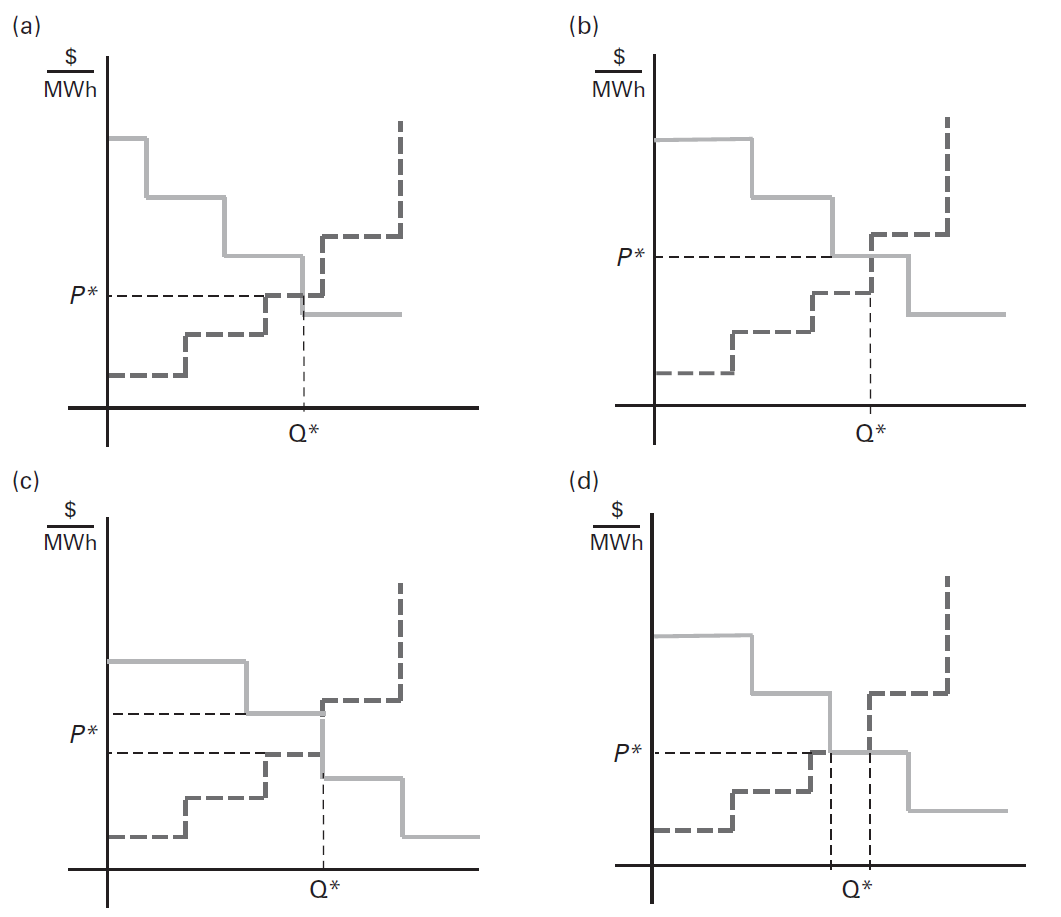
\includegraphics[scale=.35]{figure/eq.png}
    \caption{As Quatro Possibilidades de Equilíbrio de Mercado}
    \label{fig:eq}
\end{figure}

\subsection{Equivalência entre Problemas}
Note que os resultados do Problema da Firma, Problema do Consumidor e do Problema do Planejador Central são extremamente parecidos. Em específico note que $\mu$ age como o análogo do preço no problema do planejador central.

Essa semelhança não é surpreendente e decorre do chamado "Primeiro Teorema do Bem-Estar", que enuncia as condições (aqui atendidas) para que o equilíbrio de mercado competitivo seja idêntico ao equilíbrio do planejador central - ou do monopolista perfeitamente regulado (sem assimetria de informação).

\begin{teo}[Primeiro Teorema do Bem-Estar]
    Sob competição perfeita, o equilíbrio de mercado competitivo é Pareto eficiente i.e. idêntico ao equilíbrio derivado do problema do planejador central maximizador de bem-estar social.
\end{teo}

